\subsection{Rediger adgangskode}

Log ind funktionen inddeles i en grænseflade og en dertilhørende controller, som det fremgår af \autoref{fig:Designlogind}. 

\begin{figure} [H]
\centering
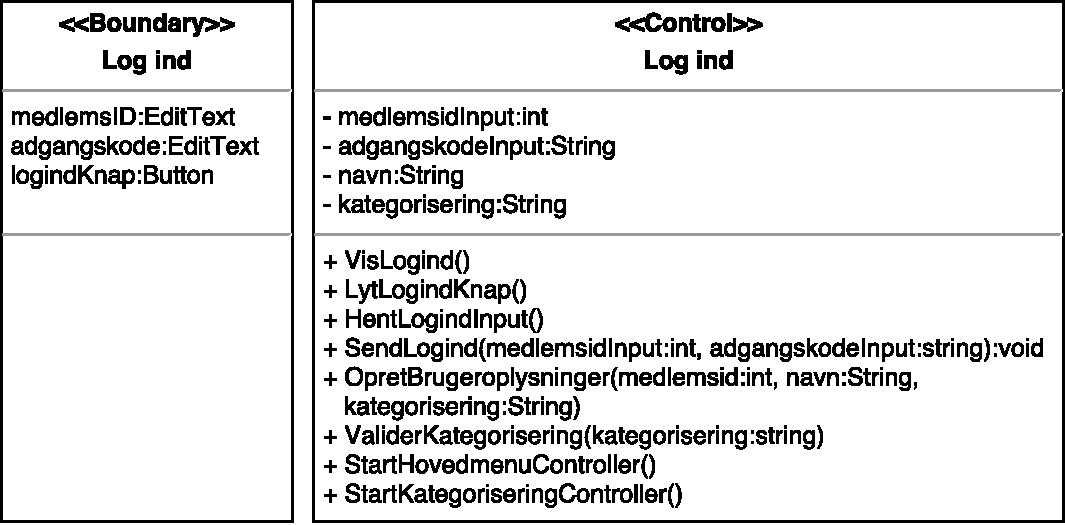
\includegraphics[width=0.9\textwidth]{figures/MVC/MVCLogInd}
\caption{Designklasser for log ind.}
\label{fig:Designlogind}
\end{figure}

I \textit{LogindGrænseflade} opstilles tekstfelter for medlemsID og adgangskode, hvor brugeren kan angive deres log ind informationer. Dertil opsættes en log ind knap, af typen button, der ved tryk indikerer, at brugerens informationer er angivet. 

Der er til \textit{LogindGrænseflade} opstillet en \textit{LogindController}, der har til formål at håndtere informationer angivet i logindgrænsefladen med databasen. Dertil vil controlleren validere indtastet log ind information med information fra databasen. Afvises log ind vises en fejlmeddelelse. Godkendes log ind hentes brugerdata fra databasen. Brugerdata omfatter brugerens oplysninger, resultater samt venneliste. Indgår kategoriseringen i brugeroplysningerne fra databasen startes hovedmenuen, hvis ikke startes kategoriseringen. 
